\documentclass[12pt,t]{beamer}
\usepackage{graphicx}
\setbeameroption{hide notes}
\setbeamertemplate{note page}[plain]
\usepackage{listings}
\usepackage{url}

% header.tex: boring LaTeX/Beamer details + macros

% get rid of junk
\usetheme{default}
\beamertemplatenavigationsymbolsempty
\hypersetup{pdfpagemode=UseNone} % don't show bookmarks on initial view


% font
\usepackage{fontspec}
\setsansfont
  [ ExternalLocation = fonts/ ,
    UprightFont = *-regular ,
    BoldFont = *-bold ,
    ItalicFont = *-italic ,
    BoldItalicFont = *-bolditalic ]{texgyreheros}
\setbeamerfont{note page}{family*=pplx,size=\footnotesize} % Palatino for notes
% "TeX Gyre Heros can be used as a replacement for Helvetica"
% I've placed them in fonts/; alternatively you can install them
% permanently on your system as follows:
%     Download http://www.gust.org.pl/projects/e-foundry/tex-gyre/heros/qhv2.004otf.zip
%     In Unix, unzip it into ~/.fonts
%     In Mac, unzip it, double-click the .otf files, and install using "FontBook"

% named colors
\definecolor{offwhite}{RGB}{255,250,240}
\definecolor{gray}{RGB}{155,155,155}

\ifx\notescolors\undefined % slides
  \definecolor{foreground}{RGB}{255,255,255}
  \definecolor{background}{RGB}{24,24,24}
  \definecolor{title}{RGB}{107,174,214}
  \definecolor{subtitle}{RGB}{102,255,204}
  \definecolor{hilit}{RGB}{102,255,204}
  \definecolor{vhilit}{RGB}{255,111,207}
  \definecolor{lolit}{RGB}{155,155,155}
\else % notes
  \definecolor{background}{RGB}{255,255,255}
  \definecolor{foreground}{RGB}{24,24,24}
  \definecolor{title}{RGB}{27,94,134}
  \definecolor{subtitle}{RGB}{22,175,124}
  \definecolor{hilit}{RGB}{122,0,128}
  \definecolor{vhilit}{RGB}{255,0,128}
  \definecolor{lolit}{RGB}{95,95,95}
\fi
\definecolor{nhilit}{RGB}{128,0,128}  % hilit color in notes
\definecolor{nvhilit}{RGB}{255,0,128} % vhilit for notes

\newcommand{\hilit}{\color{hilit}}
\newcommand{\vhilit}{\color{vhilit}}
\newcommand{\nhilit}{\color{nhilit}}
\newcommand{\nvhilit}{\color{nvhilit}}
\newcommand{\lolit}{\color{lolit}}

% use those colors
\setbeamercolor{titlelike}{fg=title}
\setbeamercolor{subtitle}{fg=subtitle}
\setbeamercolor{institute}{fg=lolit}
\setbeamercolor{normal text}{fg=foreground,bg=background}
\setbeamercolor{item}{fg=foreground} % color of bullets
\setbeamercolor{subitem}{fg=lolit}
\setbeamercolor{itemize/enumerate subbody}{fg=lolit}
\setbeamertemplate{itemize subitem}{{\textendash}}
\setbeamerfont{itemize/enumerate subbody}{size=\footnotesize}
\setbeamerfont{itemize/enumerate subitem}{size=\footnotesize}

% page number
\setbeamertemplate{footline}{%
    \raisebox{5pt}{\makebox[\paperwidth]{\hfill\makebox[20pt]{\lolit
          \scriptsize\insertframenumber}}}\hspace*{5pt}}

% add a bit of space at the top of the notes page
\addtobeamertemplate{note page}{\setlength{\parskip}{12pt}}

% default link color
\hypersetup{colorlinks, urlcolor={hilit}}

\ifx\notescolors\undefined % slides
  % set up listing environment
  \lstset{language=bash,
          basicstyle=\ttfamily\scriptsize,
          frame=single,
          commentstyle=,
          backgroundcolor=\color{darkgray},
          showspaces=false,
          showstringspaces=false
          }
\else % notes
  \lstset{language=bash,
          basicstyle=\ttfamily\scriptsize,
          frame=single,
          commentstyle=,
          backgroundcolor=\color{offwhite},
          showspaces=false,
          showstringspaces=false
          }
\fi

% a few macros
\newcommand{\bi}{\begin{itemize}}
\newcommand{\bbi}{\vspace{24pt} \begin{itemize} \itemsep8pt}
\newcommand{\ei}{\end{itemize}}
\newcommand{\ig}{\includegraphics}
\newcommand{\subt}[1]{{\footnotesize \color{subtitle} {#1}}}
\newcommand{\ttsm}{\tt \small}
\newcommand{\ttfn}{\tt \footnotesize}
\newcommand{\figh}[2]{\centerline{\includegraphics[height=#2\textheight]{#1}}}
\newcommand{\figw}[2]{\centerline{\includegraphics[width=#2\textwidth]{#1}}}


%%%%%%%%%%%%%%%%%%%%%%%%%%%%%%%%%%%%%%%%%%%%%%%%%%%%%%%%%%%%%%%%%%%%%%
% end of header
%%%%%%%%%%%%%%%%%%%%%%%%%%%%%%%%%%%%%%%%%%%%%%%%%%%%%%%%%%%%%%%%%%%%%%

% title info
\title{A Practical Tour of Super Learning}
\author{Nima Hejazi \inst{1} \and Evan Muzzall \inst{2}}
\institute{\inst{1} Division of Biostatistics, University of
                    California, Berkeley
           \and
           \inst{2} D-Lab, University of California, Berkeley}

\date{ \underline{slides}: \url{https://goo.gl/wWa9QC}}
\begin{document}

% title slide
{
\setbeamertemplate{footline}{} % no page number here
\frame{
  \titlepage

  \vfill \hfill 
\includegraphics[height=6mm]{Figs/cc-zero.png} \vspace*{-1cm}

  \note{These are slides from a presentation on practical ensemble learning with
    the Super Learner and h2oEnsemble packages for the R language, most
    recently presented at a meeting of The Hacker Within, at the Berkeley
    Institute for Data Science at UC Berkeley, on 6 December 2016.

    source: {\tt https://github.com/nhejazi/talk-h2oSL-THW-2016} \\
    slides: {\tt https://goo.gl/CXC2FF} \\
    with notes: {\tt http://goo.gl/wWa9QC}
}
}
}


\begin{frame}[fragile,c]{1. Ensemble Learning -- What?}

\begin{center}
\begin{minipage}[c]{9.3cm}
\begin{semiverbatim}
\lstset{basicstyle=\normalsize}
\begin{lstlisting}[linewidth=10.0cm]
 In statistics and machine learning,
 ensemble methods use multiple
 learning algorithms to obtain better
 predictive performance than could be
 obtained from any of the constituent
 learning algorithms alone.

 - Wikipedia, November 2016
\end{lstlisting}
\end{semiverbatim}
\end{minipage}
\end{center}

\note{
  This rather elementary definition of ``ensemble learning'' encapsulates quite
  well the core notions necessary to understand why we might be interested in
  optimizing such procedures. In particular, we will see that a weighted
  collection of individual learning algorithms can not only outperform other
  algorithms in practice but also has been shown to be theoretically optimal.
}
\end{frame}


\begin{frame}[c]{2. Ensemble Learning -- Why?}

\vspace*{3mm}

\centering

  \begin{itemize}
    \itemsep12pt
    \item Ensemble methods outperform individual (base) learning algorithms.
    \item By combining a set of individual learning algorithms using a
          \textit{metalearning} algorithm, ensemble methods can approximate
          complex functional relationships.
    \item When the true functional relationship is not in the set of base
          learning algorithms, ensemble methods approximate the true function
          well.
    \item \textit{n.b.}, ensemble methods can, even asymptotically, perform only
          as well as the best weighted combination of the candidate learners.
  \end{itemize}
\note{
  A variety of techniques exist for ensemble learning, ranging from the classic
  ``random forest'' (of Leo Breiman) to ``xgboost'' to ``Super Learner'' (van
  der Laan \textit{et al.}). In this talk, we will focus on the elementary
  theoretical properties of ``Super Learner'', with an eye towards application.

  Theoretically, a range of different algorithms can be used in the metalearning
  step; however, in practice, often, logistic regression is used.
}
\end{frame}


\begin{frame}[c]{3. Ensemble Learning -- How?}

\vspace*{3mm}

\textit{Common strategies for performing ensemble learning:}

\vspace{1em}

\centering

  \begin{itemize}
    \itemsep12pt
    \item \underline{\textbf{Bagging}} -- reduces variance and increases
          accuracy; robust against outliers; often used with decision trees
          (\textit{i.e.}, Random Forest).
    \item \underline{\textbf{Boosting}} -- reduces variance and increases
          accuracy; not robust against outliers or noise; accomodates any loss
          function.
    \item \underline{\textbf{Stacking}} -- used in combining ``strong''
          learners; requires a \textit{metalearning} algorithm to combine the
          set of learners.
  \end{itemize}

\note{
  While a number of different strategies exist for combining various types of
  learning algorithms, most modern methods rely on stacking to produce powerful
  ensemble learners. These sorts of ensemble learners are what you want to use
  to win Kaggle competitions!
}
\end{frame}


\begin{frame}[c]{4. Introduction to Super Learner}

\vspace*{3mm}

\centering

  \begin{itemize}
    \itemsep12pt
    \item 1996 paper ``Stacked Regressions'' (L. Breiman) introduced the notion
          of model stacking using k-fold cross-validation, the precursor to the
          modern Super Learner algorithm.
    \item 2007 paper ``Super Learner'' (van der Laan \textit{et al.}) worked out
          theoretical details on the optimality of stacking. Before this, the
          reasons for the superb performance of stacking were unknown.
    \item The Super Learner algorithm learns the optimal combination of the
          base learner fits in a manner that is provably asymptotic optimal.
  \end{itemize}

\note{
  The Super Learner algorithm allows researchers to use multiple algorithms to
  outperform a single algorithm in realistic non-parametric and semi-parametric
  statistical models that are based on actual knowledge.

  The term algorithm is used very loosely to describe any mapping from the data
  into a predictor. This can range from a simple logistic regression to more
  complex algorithms such as neural nets.
}
\end{frame}


\begin{frame}[c]{5. Interlude: Cross-Validation}

\vspace*{2mm}

\centering

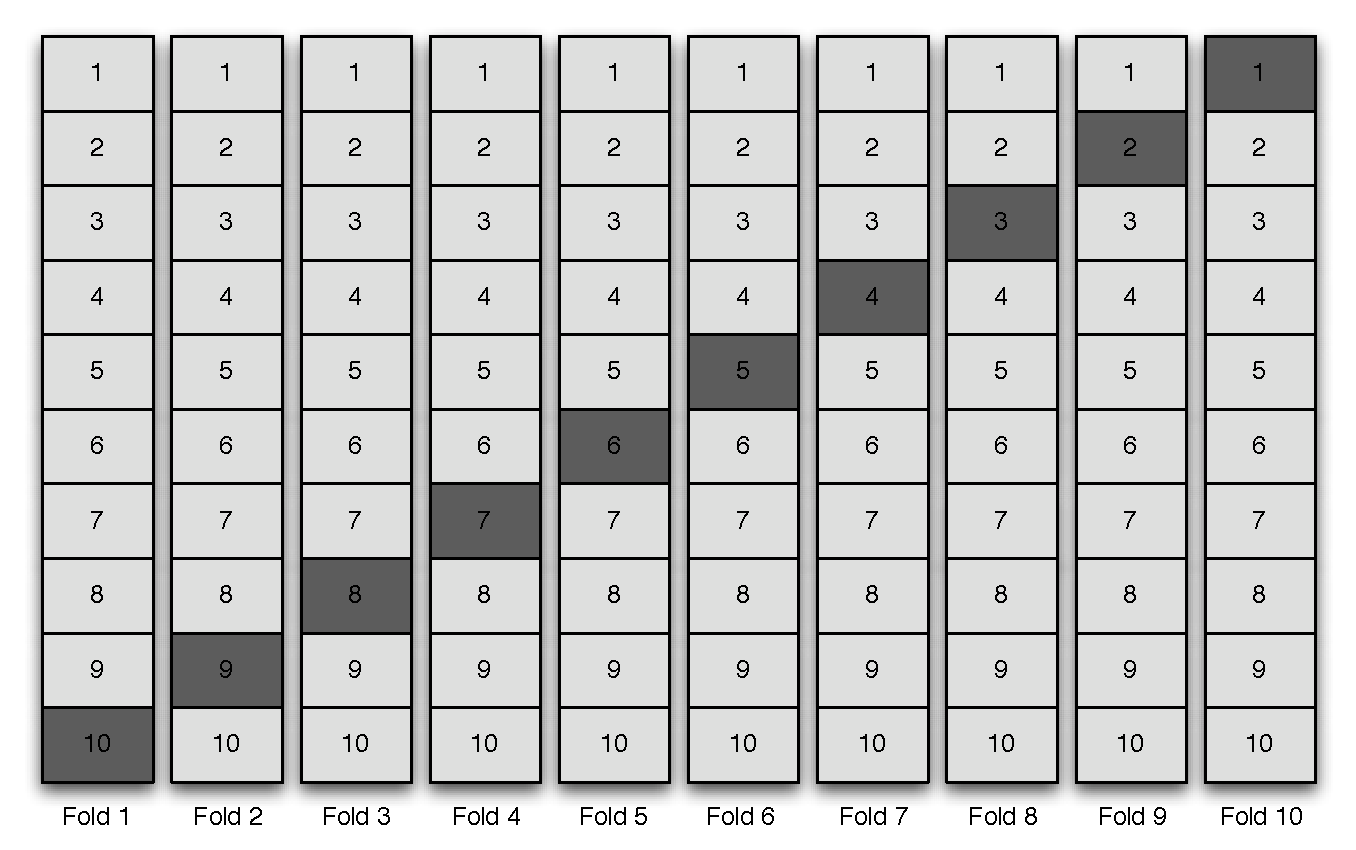
\includegraphics[scale=0.45]{Figs/cv.pdf}

\textit{The validation set rotates V times such that each set is used as the
validation set once.}

\note{
  Cross-validation solves the problem of having many algorithms, and not
  knowing which one to use and helps us avoid overfitting.

  For any given fold, $V − 1$ sets will comprise the training set and the
  remaining $1$ set is the validation set.

  The observations in the training set are used to construct (or train) the
  candidate estimators.

  The observations in the validation set are used to assess the performance
  (\textit{i.e.}, risk) of the candidate algorithms.
}
\end{frame}


\begin{frame}[c]{6. Optimality of Super Learner}

\vspace*{1mm}

\centering

  For a random variable $O = (W, A, Y)$, let the \textbf{oracle selector} be a
  rule that picks the algorithm with the lowest cross-validated risk under the
  \textit{true probability distribution} $P_{0}$. The \textbf{oracle selector}
  is unknown because it depends on observed data \underline{and} the truth.

\vspace{1em}

  Asymptotic results prove that in realistic scenarios (where none of the
  algorithms represent the true relationship), the ``discrete super learner''
  performs \textit{asymptotically as well as} the oracle selector (the best
  estimator given the algorithms in the collection).

\note{
  To clarify, theory shows that that the discrete super learner performs as
  well as the oracle selector, up to a second order term. The loss function
  must be bounded, and then we will perform as well as the algorithm that is
  the risk minimizer of the expected loss function. The number of algorithms in
  the library can grow with sample size.
}
\end{frame}


\begin{frame}[c]{7. The Discrete Super Learner}

\vspace*{3mm}

\centering

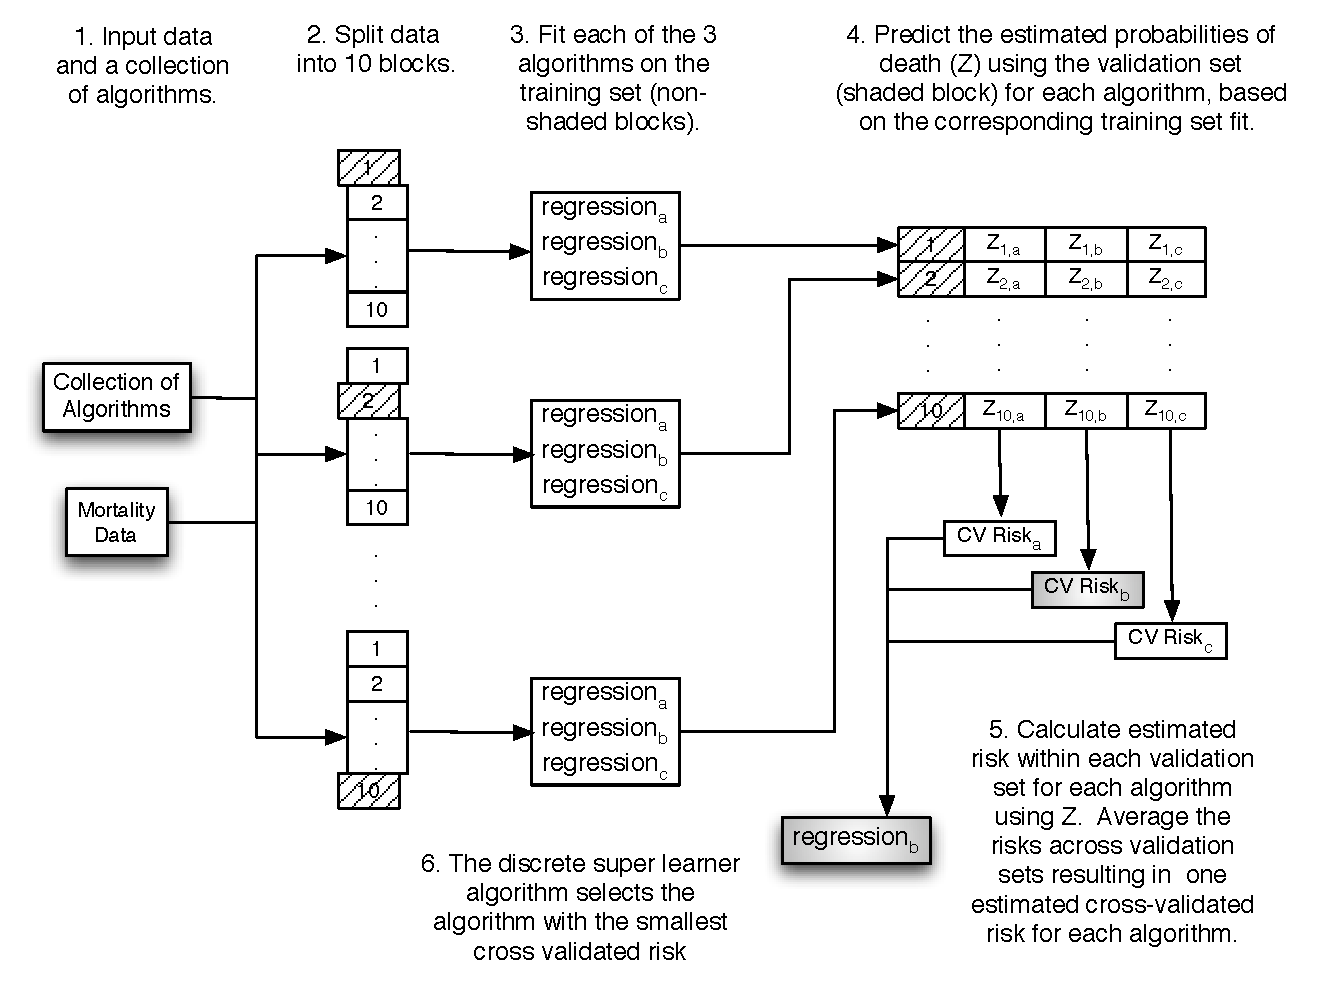
\includegraphics[scale=0.45]{Figs/discreteSL.pdf}

\note{
}
\end{frame}


\begin{frame}[c]{8. The Super Learner Algorithm}

\vspace*{3mm}

\centering

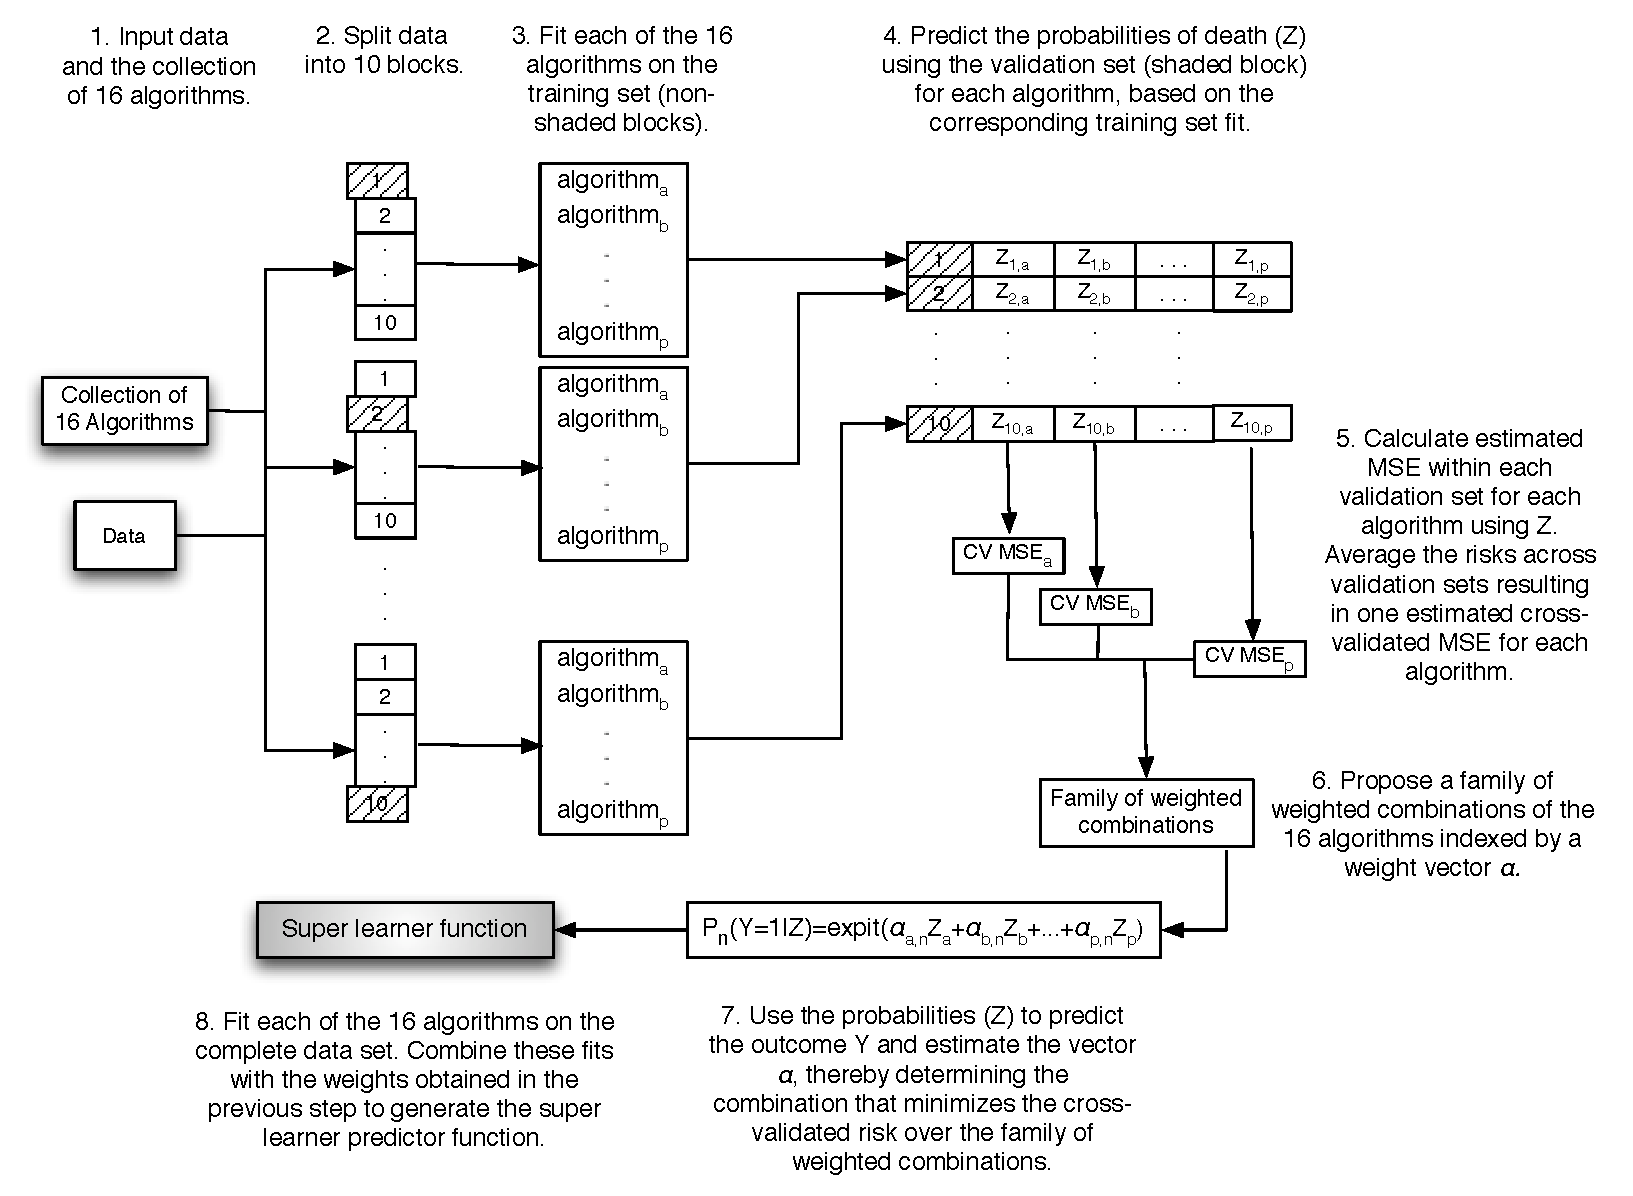
\includegraphics[scale=0.4]{Figs/SL.pdf}

\note{
  \textit{Cross-validate Base Learners:}
    \begin{itemize}
      \itemsep10pt
      \item Perform k-fold cross-validation on each learner and collect the
            cross-validated predicted values from each of the $L$ algorithms.
      \item The $N$ cross-validated predicted values from each of the $L$
            algorithms can be combined to form a new $N \times L$ matrix. Call
            this matrix, with the original response vector, ``level-one'' data.
    \end{itemize}

  \textit{Metalearning:}
    \begin{itemize}
      \itemsep10pt
      \item Train the metalearning algorithm on the ``level-one'' data.
      \item Train each of the $L$ base algorithms on the full training set.
      \item The ``ensemble model'' consists of the $L$ base learning models and
            the metalearning model, which can be used to generate predictions on
            a test set.
    \end{itemize}
}
\end{frame}


\begin{frame}[c]{9. R Package: ``SuperLearner''}

\vspace*{3mm}

\centering

  \begin{itemize}
    \itemsep12pt
    \item Implements the Super Learner prediction method (stacking) and
          contains a library of prediction algorithms to be used in the Super
          Learner.
    \item Provides a clean interface to numerous algorithms in R and defines a
          consistent API for extensibility.
  \end{itemize}

\note{
}
\end{frame}


\begin{frame}{10. R Package: ``h2oEnsemble''}

\vspace*{3mm}

\centering

\textit{Extension to the ``h2o'' R package that allows the user to train an
ensemble in the H2O cluster using any of the supervised machine learning
algorithms in H2O.}

\vspace{1em}

  \begin{itemize}
    \itemsep12pt
    \item Uses data-distributed and parallelized Java-based algorithms for the
          ensemble.
    \item All training and data processing are performed in the
          high-performance H2O cluster.
    \item Supports regression and binary classification.
  \end{itemize}

\note{
}
\end{frame}


\begin{frame}[c]{Summary}

  \begin{enumerate}
  \itemsep12pt
    \item Ensemble methods combine individual learning algorithms to approximate
          complex relationships.
    \item Super Learning (stacking) represents an optimal system for combining
          individual learning algorithms into an ensemble learner.
    \item The ``SuperLearner'' R package provides a well-maintained
          implementation of the the Super Learner algorithm.
    \item The ``h2oEnsemble'' R package provides access to a range of ensemble
          methods, developed by \href{http://www.h2o.ai}{\tt H2O.ai}.
  \end{enumerate}

  \note{
    Just a summary of what we discussed today.
}
\end{frame}


\begin{frame}[c]{}

\Large

Slides: \url{http://goo.gl/wWa9QC} \quad

\includegraphics[height=5mm]{Figs/cc-zero.png}

\vspace{10mm}

\href{https://github.com/nhejazi/talk-h2oSL-THW-2016}
{\tt GitHub: nhejazi/talk-h2oSL-THW-2016}

\note{
  Here's where you can find the resources prepared for this talk.
}
\end{frame}


\end{document}
